%=======================+=========================
%================   Detector Overview ================
%=================================================

\section[Detector overview (Curtis)]{Detector overview \label{sec:overview}}
The design of the GlueX detector \cite{Ghoul:2015ifw} is based on a solenoidal magnet that surrounds all detectors in the central region, providing a magnetic field of about $2$~T along the direction of the photon beam, which impinges on a 
$30$~cm-long liquid hydrogen target.  A schematic of the detector including its major sub-detectors is given in Fig.\,\ref{fig:gluexsketch}.
\begin{figure}[tbp]
\begin{center}
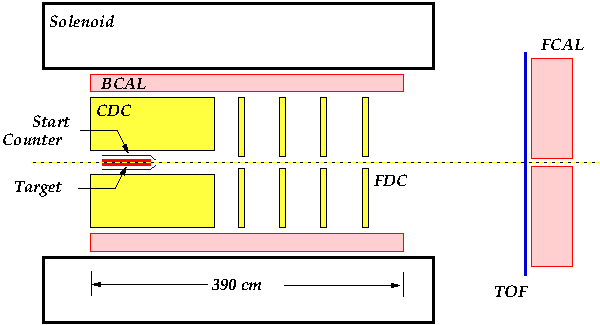
\includegraphics[width=0.7\textwidth]{figures/GlueX_Sketch.pdf}  
\caption{\label{fig:gluexsketch}          
  Sketch of GlueX detector.  The main systems of the detector are the Start Counter \cite{hdnote3064}, the Central Drift Chamber (CDC) \cite{VanHaarlem:2010yq} the Forward Drift Chamber (FDC) \cite{Pentchev2017281}, a scintillator-based Time of Flight (TOF) wall and a lead-glass Forward Calorimeter (FCAL) \cite{MORIYA201360}. The Barrel Calorimeter (BCAL) is sandwiched between the drift chambers and the inner radius of the solenoid.  (Color online)
}   
\end{center}  
\end{figure}
